\begin{landscape}
\begin{figurels}[!]
    \centering
    \caption{Singles spectra of $^{156}$Gd. Spectra are labeled with the particles being detected, the energies of the $\gamma$ and electron spectra aligned for identification. In the $\gamma$ spectrum, several lines of note are labeled. The large peak in the electron spectrum at low energy is cut off due to the threshold. It is a combination of background and the 89L peak. Transitions in the higher energy regime of the $\gamma$ spectrum cannot be determined without gating, due to additional background from the experimental room. The electron spectrum only goes to 1250 keV, as that is the limit of the detectors.}
    \label{fig:156_Singles}
\end{figurels}
\begin{figurels}[!]
    \centering
    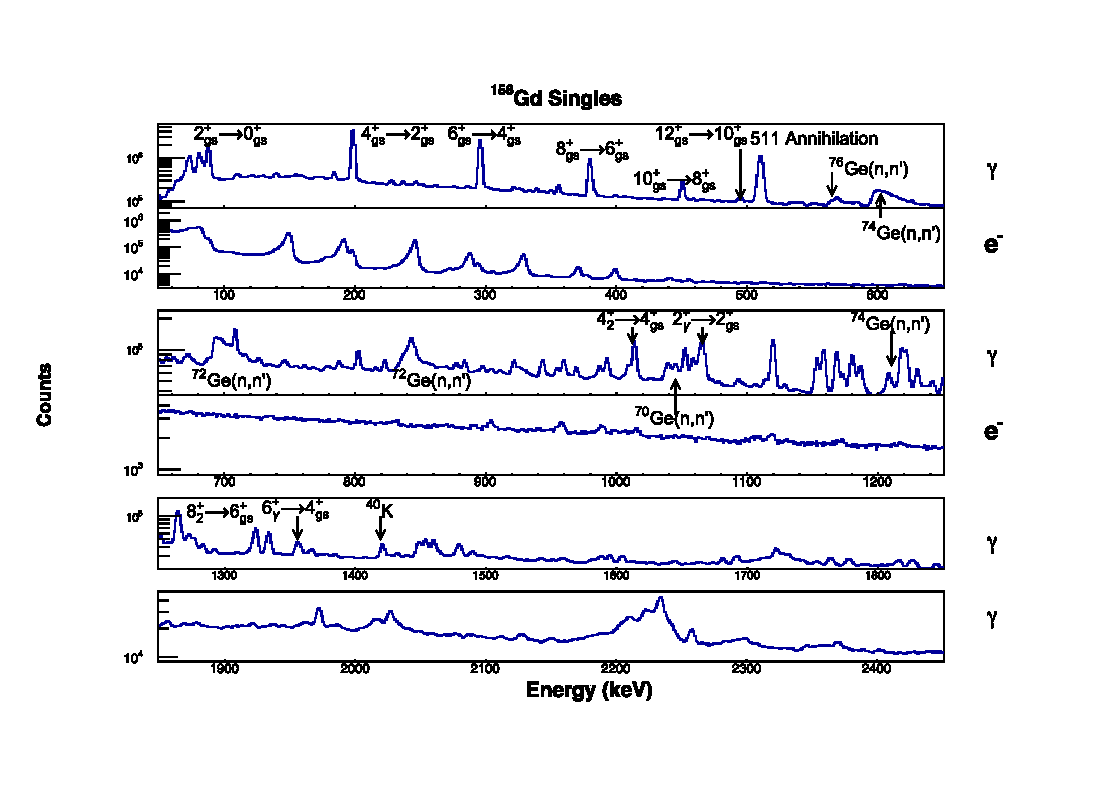
\includegraphics[scale=0.9]{156GdTablesAndFigs/156Gd_Singles_Label.eps}
\end{figurels}
\end{landscape}